\lettrine[lhang=0.17]{I}{n mathematics we have} various ways of saying that one thing is like
another. The strictest is equality. Two things are equal if there is no
way to distinguish one from another. One can be substituted for the
other in every imaginable context. For instance, did you notice that we
used \newterm{equality} of morphisms every time we talked about commuting
diagrams? That's because morphisms form a set (hom-set) and set elements
can be compared for equality.

But equality is often too strong. There are many examples of things
being the same for all intents and purposes, without actually being
equal. For instance, the pair type \code{(Bool, Char)} is not
strictly equal to \code{(Char, Bool)}, but we understand that they
contain the same information. This concept is best captured by an
\newterm{isomorphism} between two types --- a morphism that's invertible.
Since it's a morphism, it preserves the structure; and being ``iso''
means that it's part of a round trip that lands you in the same spot, no
matter on which side you start. In the case of pairs, this isomorphism
is called \code{swap}:

\begin{Verbatim}
swap :: (a,b) -> (b,a)
swap (a,b) = (b,a)
\end{Verbatim}
\code{swap} happens to be its own inverse.

\section{Adjunction and Unit/Counit Pair}

When we talk about categories being isomorphic, we express this in terms
of mappings between categories, a.k.a. functors. We would like to be
able to say that two categories $\cat{C}$ and $\cat{D}$ are isomorphic if
there exists a functor $R$ (``right'') from $\cat{C}$ to $\cat{D}$,
which is invertible. In other words, there exists another functor
$L$ (``left'') from $\cat{D}$ back to $\cat{C}$ which, when
composed with $R$, is equal to the identity functor $I$.
There are two possible compositions, $R \circ L$ and
$L \circ R$; and two possible identity functors: one in $\cat{C}$
and another in $\cat{D}$.

\begin{figure}[H]
\centering
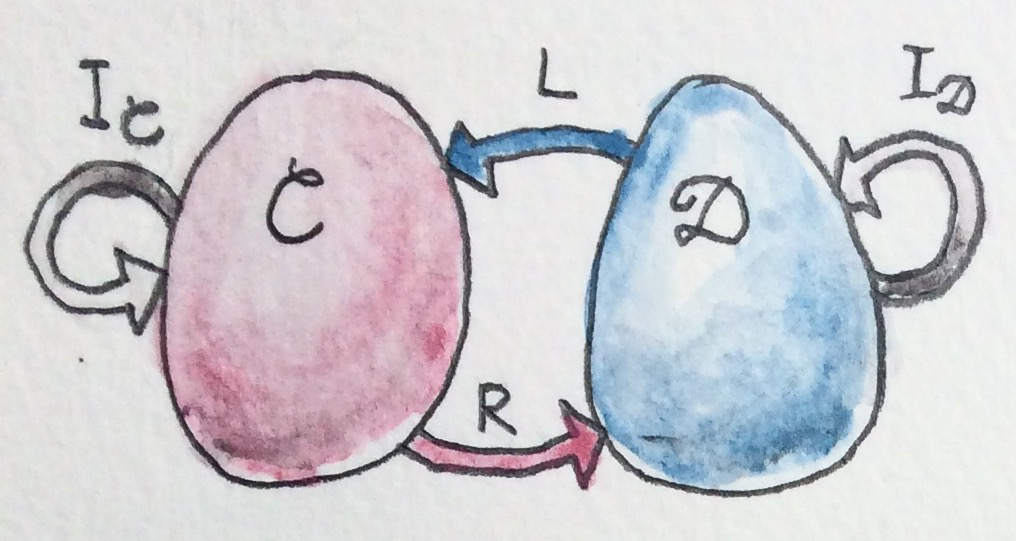
\includegraphics[width=3.12500in]{images/adj-1.jpg}
\end{figure}

\noindent
But here's the tricky part: What does it mean for two functors to be
\emph{equal}? What do we mean by this equality:
\[R \circ L = I_{\cat{D}}\]
or this one:
\[L \circ R = I_{\cat{C}}\]
It would be reasonable to define functor equality in terms of equality
of objects. Two functors, when acting on equal objects, should produce
equal objects. But we don't, in general, have the notion of object
equality in an arbitrary category. It's just not part of the definition.
(Going deeper into this rabbit hole of ``what equality really is,'' we
would end up in Homotopy Type Theory.)

You might argue that functors \emph{are} morphisms in the category of
categories, so they should be equality-comparable. And indeed, as long
as we are talking about small categories, where objects form a set, we
can indeed use the equality of elements of a set to equality-compare
objects.

But, remember, $\Cat$ is really a $\cat{2}$-category. Hom-sets in a
$\cat{2}$-category have additional structure --- there are $2$-morphisms acting
between $1$-morphisms. In $\Cat$, $1$-morphisms are functors, and
$2$-morphisms are natural transformations. So it's more natural (can't
avoid this pun!) to consider natural isomorphisms as substitutes for
equality when talking about functors.

So, instead of isomorphism of categories, it makes sense to consider a
more general notion of \newterm{equivalence}. Two categories $\cat{C}$ and
$\cat{D}$ are \emph{equivalent} if we can find two functors going back
and forth between them, whose composition (either way) is
\newterm{naturally isomorphic} to the identity functor. In other words,
there is a two-way natural transformation between the composition
$R \circ L$ and the identity functor $I_{\cat{D}}$, and another
between $L \circ R$ and the identity functor $I_{\cat{C}}$.

Adjunction is even weaker than equivalence, because it doesn't require
that the composition of the two functors be \emph{isomorphic} to the
identity functor. Instead it stipulates the existence of a \newterm{one
way} natural transformation from $I_{\cat{D}}$ to $R \circ L$, and
another from $L \circ R$ to $I_{\cat{C}}$. Here are the signatures of
these two natural transformations:
\begin{gather*}
\eta \Colon I_{\cat{D}} \to R \circ L \\
\varepsilon \Colon L \circ R \to I_{\cat{C}}
\end{gather*}
$\eta$ is called the unit, and $\varepsilon$ the counit of the adjunction.

Notice the asymmetry between these two definitions. In general, we don't
have the two remaining mappings:
\begin{gather*}
R \circ L \to I_{\cat{D}} \quad\quad\text{not necessarily} \\
I_{\cat{C}} \to L \circ R \quad\quad\text{not necessarily}
\end{gather*}
Because of this asymmetry, the functor $L$ is called the
\newterm{left adjoint} to the functor $R$, while the functor
$R$ is the right adjoint to $L$. (Of course, left and
right make sense only if you draw your diagrams one particular way.)

The compact notation for the adjunction is:
\[L \dashv R\]
To better understand the adjunction, let's analyze the unit and the
counit in more detail.

\begin{figure}[H]
\centering
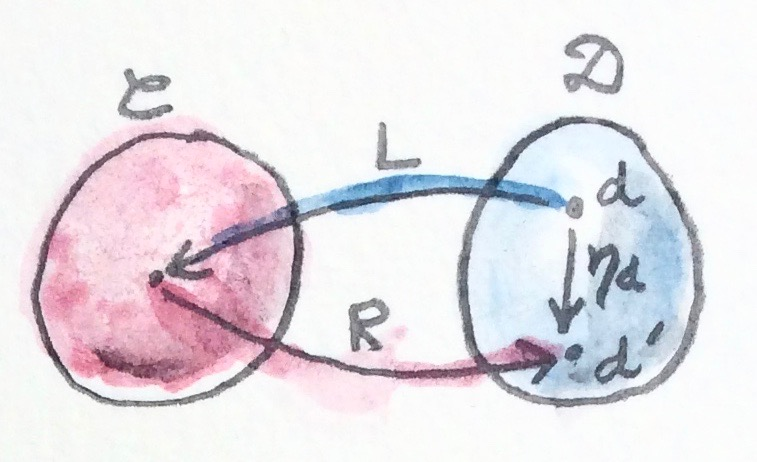
\includegraphics[width=60mm]{images/adj-unit.jpg}
\end{figure}

\noindent
Let's start with the unit. It's a natural transformation, so it's a
family of morphisms. Given an object $d$ in $\cat{D}$, the
component of $\eta$ is a morphism between $I d$, which is equal to
$d$, and $(R \circ L) d$; which, in the picture, is called
$d'$:
\[\eta_d \Colon d \to (R \circ L) d\]
Notice that the composition $R \circ L$ is an endofunctor in $\cat{D}$.

This equation tells us that we can pick any object $d$ in
$\cat{D}$ as our starting point, and use the round trip functor
$R \circ L$ to pick our target object $d'$. Then we
shoot an arrow --- the morphism $\eta_d$ --- to our target.

\begin{figure}[H]
\centering
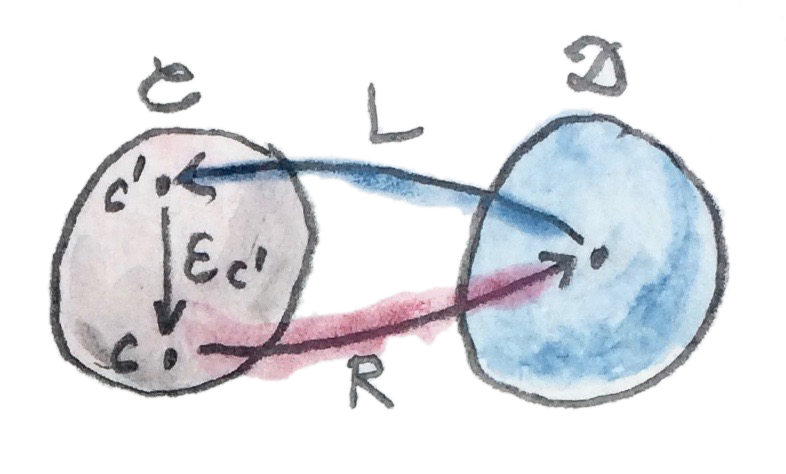
\includegraphics[width=60mm]{images/adj-counit.jpg}
\end{figure}

\noindent
By the same token, the component of the counit ε can be described as:
\[\varepsilon_{c'} \Colon (L \circ R) c \to c\]
where $c'$ is $(L \circ R) c$. It tells us that we
can pick any object $c$ in $\cat{C}$ as our target, and use the
round trip functor $L \circ R$ to pick the source
$c'$. Then we shoot the arrow --- the morphism
$\varepsilon_{c'}$ --- from the source to the target.

Another way of looking at unit and counit is that unit lets us
\emph{introduce} the composition $R \circ L$ anywhere we could
insert an identity functor on $\cat{D}$; and counit lets us
\emph{eliminate} the composition $L \circ R$, replacing it with the
identity on $\cat{C}$. That leads to some ``obvious'' consistency
conditions, which make sure that introduction followed by elimination
doesn't change anything:
\begin{gather*}
L = L \circ I_{\cat{D}} \to L \circ R \circ L \to I_{\cat{C}} \circ L = L \\
R = I_{\cat{D}} \circ R \to R \circ L \circ R \to R \circ I_{\cat{C}} = R
\end{gather*}
These are called triangular identities because they make the following
diagrams commute:

\begin{figure}[H]
  \centering

  \begin{subfigure}
    \centering
    \begin{tikzcd}[column sep=large, row sep=large]
    	L \arrow[rd, equal] \arrow[r, "L \circ \eta"] 
          & L \circ R \circ L \arrow[d, "\epsilon \circ L"] \\
    	    & L
    \end{tikzcd}
  \end{subfigure}%
  \hspace{1cm}
  \begin{subfigure}
    \centering
    \begin{tikzcd}[column sep=large, row sep=large]
      R \arrow[rd, equal] \arrow[r, "\eta \circ R"] 
          & R \circ L \circ R \arrow[d, "R \circ \epsilon"] \\
          & R
    \end{tikzcd}
  \end{subfigure}
\end{figure}

\noindent
These are diagrams in the functor category: the arrows are natural
transformations, and their composition is the horizontal composition of
natural transformations. In components, these identities become:
\begin{gather*}
\varepsilon_{L d} \circ L \eta_d = \id_{L d} \\
R \varepsilon_c \circ \eta_{R c} = \id_{R c}
\end{gather*}
We often see unit and counit in Haskell under different names. Unit is
known as \code{return} (or \code{pure}, in the definition of
\code{Applicative}):

\begin{Verbatim}
return :: d -> m d
\end{Verbatim}
and counint as \code{extract}:

\begin{Verbatim}
extract :: w c -> c
\end{Verbatim}
Here, \code{m} is the (endo-) functor corresponding to $R \circ L$,
and \code{w} is the (endo-) functor corresponding to $L \circ R$. As
we'll see later, they are part of the definition of a monad and a
comonad, respectively.

If you think of an endofunctor as a container, the unit (or
\code{return}) is a polymorphic function that creates a default box
around a value of arbitrary type. The counit (or \code{extract}) does
the reverse: it retrieves or produces a single value from a container.

We'll see later that every pair of adjoint functors defines a monad and
a comonad. Conversely, every monad or comonad may be factorized into a
pair of adjoint functors --- this factorization is not unique, though.

In Haskell, we use monads a lot, but only rarely factorize them into
pairs of adjoint functors, primarily because those functors would
normally take us out of $\cat{Hask}$.

We can however define adjunctions of \newterm{endofunctors} in Haskell.
Here's part of the definition taken from
\code{Data.Functor.Adjunction}:

\begin{Verbatim}
class (Functor f, Representable u) =>
      Adjunction f u | f -> u, u -> f where
    unit :: a -> u (f a)
    counit :: f (u a) -> a
\end{Verbatim}
This definition requires some explanation. First of all, it describes a
multi-parameter type class --- the two parameters being \code{f} and
\code{u}. It establishes a relation called \code{Adjunction} between
these two type constructors.

Additional conditions, after the vertical bar, specify functional
dependencies. For instance, \code{f -> u} means that
\code{u} is determined by \code{f} (the relation between \code{f}
and \code{u} is a function, here on type constructors). Conversely,
\code{u -> f} means that, if we know \code{u}, then
\code{f} is uniquely determined.

I'll explain in a moment why, in Haskell, we can impose the condition
that the right adjoint \code{u} be a \newterm{representable} functor.

\section{Adjunctions and Hom-Sets}

There is an equivalent definition of the adjunction in terms of natural
isomorphisms of hom-sets. This definition ties nicely with universal
constructions we've been studying so far. Every time you hear the
statement that there is some unique morphism, which factorizes some
construction, you should think of it as a mapping of some set to a
hom-set. That's the meaning of ``picking a unique morphism.''

Furthermore, factorization can be often described in terms of natural
transformations. Factorization involves commuting diagrams --- some
morphism being equal to a composition of two morphisms (factors). A
natural transformation maps morphisms to commuting diagrams. So, in a
universal construction, we go from a morphism to a commuting diagram,
and then to a unique morphism. We end up with a mapping from morphism to
morphism, or from one hom-set to another (usually in different
categories). If this mapping is invertible, and if it can be naturally
extended across all hom-sets, we have an adjunction.

The main difference between universal constructions and adjunctions is
that the latter are defined globally --- for all hom-sets. For instance,
using a universal construction you can define a product of two select
objects, even if it doesn't exist for any other pair of objects in that
category. As we'll see soon, if the product of \emph{any pair} of
objects exists in a category, it can be also defined through an
adjunction.

\begin{figure}[H]
\centering
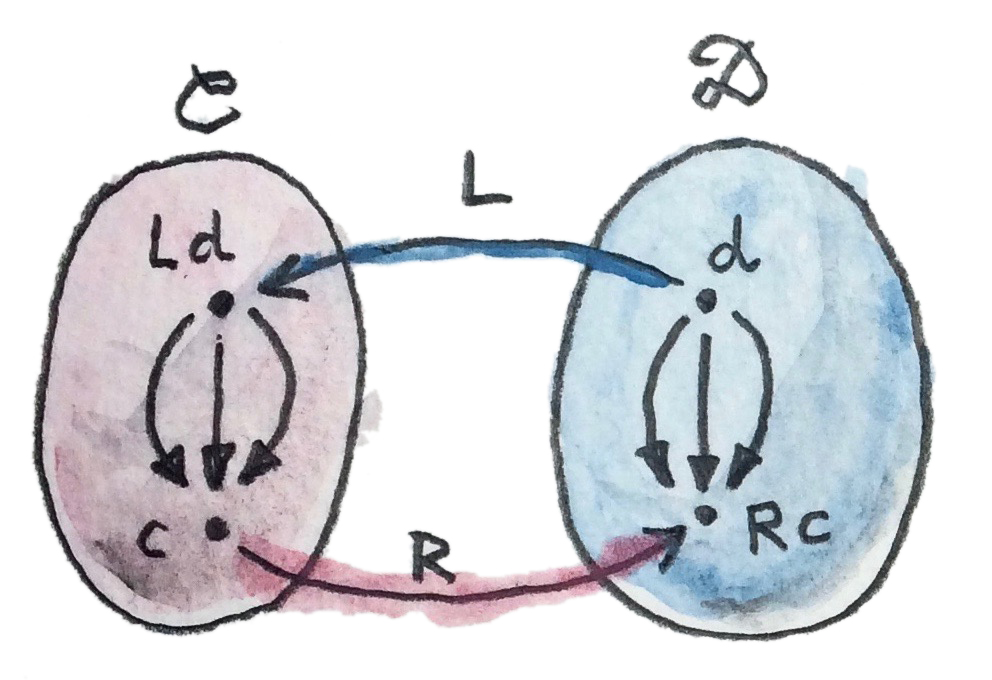
\includegraphics[width=60mm]{images/adj-homsets.jpg}
\end{figure}

\noindent
Here's the alternative definition of the adjunction using hom-sets. As
before, we have two functors $L \Colon \cat{D} \to \cat{C}$ and
$R \Colon \cat{C} \to \cat{D}$. We pick two arbitrary objects: the
source object $d$ in $\cat{D}$, and the target object $c$
in $\cat{C}$. We can map the source object $d$ to $\cat{C}$ using
$L$. Now we have two objects in $\cat{C}$, $L d$ and
$c$. They define a hom-set:
\[\cat{C}(L d, c)\]
Similarly, we can map the target object $c$ using $R$. Now
we have two objects in $\cat{D}$, $d$ and $R c$. They,
too, define a hom set:
\[\cat{D}(d, R c)\]
We say that $L$ is left adjoint to $R$ iff there is an
isomorphism of hom sets:
\[\cat{C}(L d, c) \cong \cat{D}(d, R c)\]
that is natural both in $d$ and $c$.
Naturality means that the source $d$ can be varied smoothly
across $\cat{D}$; and the target $c$, across $\cat{C}$. More
precisely, we have a natural transformation $\varphi$ between the
following two (covariant) functors from $\cat{C}$ to $\Set$. Here's
the action of these functors on objects:
\begin{gather*}
c \to \cat{C}(L d, c) \\
c \to \cat{D}(d, R c)
\end{gather*}
The other natural transformation, $\psi$, acts between the following
(contravariant) functors:
\begin{gather*}
d \to \cat{C}(L d, c) \\
d \to \cat{D}(d, R c)
\end{gather*}
Both natural transformations must be invertible.

It's easy to show that the two definitions of the adjunction are
equivalent. For instance, let's derive the unit transformation starting
from the isomorphism of hom-sets:
\[\cat{C}(L d, c) \cong \cat{D}(d, R c)\]
Since this isomorphism works for any object $c$, it must also
work for $c = L d$:
\[\cat{C}(L d, L d) \cong \cat{D}(d, (R \circ L) d)\]
We know that the left hand side must contain at least one morphism, the
identity. The natural transformation will map this morphism to an
element of $\cat{D}(d, (R \circ L) d)$ or, inserting the identity
functor $I$, a morphism in:
\[\cat{D}(I d, (R \circ L) d)\]
We get a family of morphisms parameterized by $d$. They form a
natural transformation between the functor $I$ and the functor
$R \circ L$ (the naturality condition is easy to verify). This is
exactly our unit, $\eta$.

Conversely, starting from the existence of the unit and co-unit, we can
define the transformations between hom-sets. For instance, let's pick an
arbitrary morphism $f$ in the hom-set $\cat{C}(L d, c)$. We
want to define a $\varphi$ that, acting on $f$, produces a
morphism in $\cat{D}(d, R c)$.

There isn't really much choice. One thing we can try is to lift
$f$ using $R$. That will produce a morphism $R f$
from $R (L d)$ to $R c$ --- a morphism that's an
element of $\cat{D}((R \circ L) d, R c)$.

What we need for a component of $\varphi$, is a morphism from
$d$ to $R c$. That's not a problem, since we can use a
component of $\eta_d$ to get from $d$ to
$(R \circ L) d$. We get:
\[\varphi_f = R f \circ \eta_d\]
The other direction is analogous, and so is the derivation of $\psi$.

Going back to the Haskell definition of \code{Adjunction}, the natural
transformations $\varphi$ and $\psi$ are replaced by polymorphic
(in \code{a} and \code{b}) functions \code{leftAdjunct} and
\code{rightAdjunct}, respectively. The functors $L$ and
$R$ are called \code{f} and \code{u}:

\begin{Verbatim}
class (Functor f, Representable u) => 
  Adjunction f u | f -> u, u -> f where
    leftAdjunct  :: (f a -> b) -> (a -> u b)
    rightAdjunct :: (a -> u b) -> (f a -> b) 
\end{Verbatim}
The equivalence between the \code{unit}/\code{counit} formulation
and the\\ \code{leftAdjunct}/\code{rightAdjunct} formulation is
witnessed by these mappings:

\begin{Verbatim}
unit           = leftAdjunct id
counit         = rightAdjunct id
leftAdjunct f  = fmap f . unit
rightAdjunct f = counit . fmap f
\end{Verbatim}
It's very instructive to follow the translation from the categorical
description of the adjunction to Haskell code. I highly encourage this
as an exercise.

We are now ready to explain why, in Haskell, the right adjoint is
automatically a \hyperref[representable-functors]{representable
functor}. The reason for this is that, to the first approximation, we
can treat the category of Haskell types as the category of sets.

When the right category $\cat{D}$ is $\Set$, the right adjoint
$R$ is a functor from $\cat{C}$ to $\Set$. Such a functor is
representable if we can find an object $rep$ in $\cat{C}$ such
that the hom-functor $\cat{C}(rep, \_)$ is naturally isomorphic to
$R$. It turns out that, if $R$ is the right adjoint of
some functor $L$ from $\Set$ to $\cat{C}$, such an object
always exists --- it's the image of the singleton set $()$ under
$L$:
\[rep = L ()\]
Indeed, the adjunction tells us that the following two hom-sets are
naturally isomorphic:
\[\cat{C}(L (), c) \cong \Set((), R c)\]
For a given $c$, the right hand side is the set of functions from
the singleton set $()$ to $R c$. We've seen earlier that
each such function picks one element from the set $R\ c$. The set
of such functions is isomorphic to the set $R c$. So we have:
\[\cat{C}(L (), -) \cong R\]
which shows that $R$ is indeed representable.

\section{Product from Adjunction}

We have previously introduced several concepts using universal
constructions. Many of those concepts, when defined globally, are easier
to express using adjunctions. The simplest non-trivial example is that
of the product. The gist of the \hyperref[products-and-coproducts]{universal
construction of the product} is the ability to factorize any
product-like candidate through the universal product.

More precisely, the product of two objects $a$ and $b$ is
the object $(a\times{}b)$ (or \code{(a, b)} in the Haskell
notation) equipped with two morphisms $fst$ and $snd$ such
that, for any other candidate $c$ equipped with two morphisms
$p \Colon c \to a$ and $q \Colon c \to b$, there
exists a unique morphism $m \Colon c \to (a, b)$ that
factorizes $p$ and $q$ through $fst$ and $snd$.

As we've seen earlier, in Haskell, we can implement a \code{factorizer} that generates this
morphism from the two projections:

\begin{Verbatim}
factorizer :: (c -> a) -> (c -> b) -> (c -> (a, b))
factorizer p q = \x -> (p x, q x)
\end{Verbatim}
It's easy to verify that the factorization conditions hold:

\begin{Verbatim}
fst . factorizer p q = p
snd . factorizer p q = q
\end{Verbatim}
We have a mapping that takes a pair of morphisms \code{p} and
\code{q} and produces another morphism
\code{m = factorizer p q}.

How can we translate this into a mapping between two hom-sets that we
need to define an adjunction? The trick is to go outside of
\textbf{Hask} and treat the pair of morphisms as a single morphism in
the product category.

Let me remind you what a product category is. Take two arbitrary
categories $\cat{C}$ and $\cat{D}$. The objects in the product category
$\cat{C}\times{}\cat{D}$ are pairs of objects, one from $\cat{C}$ and one from
$\cat{D}$. The morphisms are pairs of morphisms, one from $\cat{C}$ and
one from $\cat{D}$.

To define a product in some category $\cat{C}$, we should start with the
product category $\cat{C}\times{}\cat{C}$. Pairs of morphism from $\cat{C}$ are single
morphisms in the product category $\cat{C}\times{}\cat{C}$.

\begin{figure}[H]
\centering
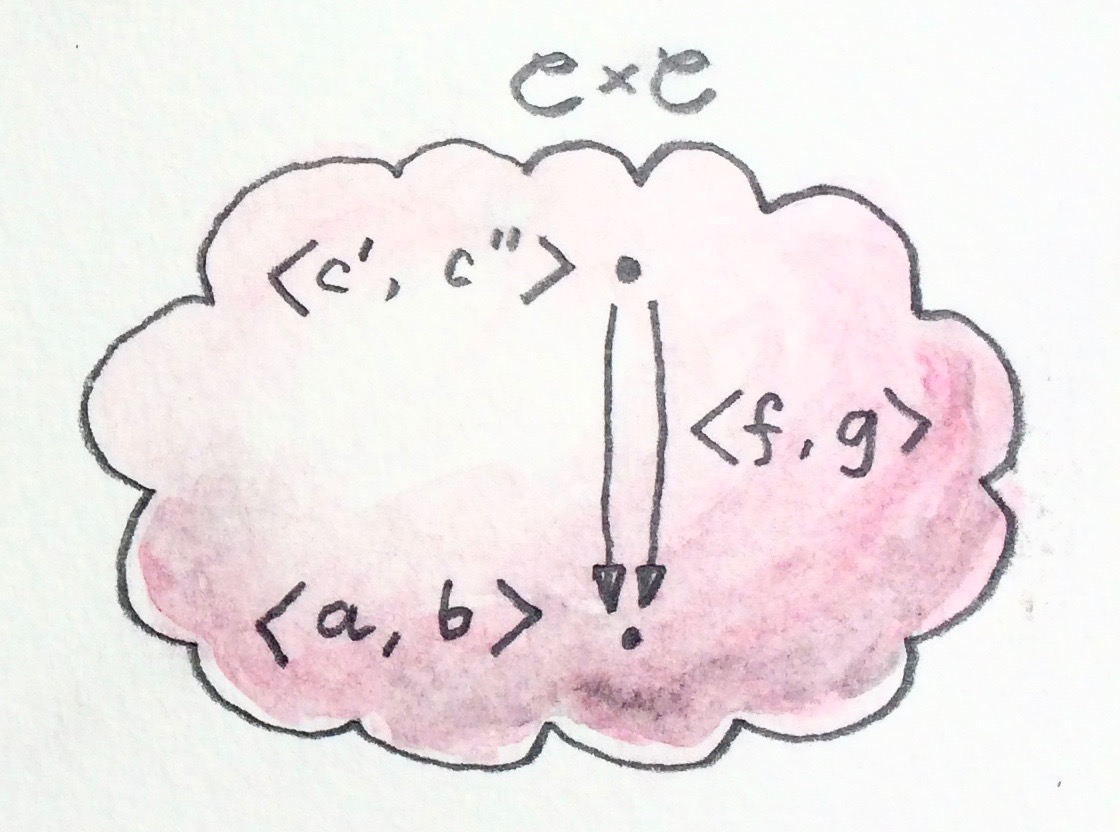
\includegraphics[width=60mm]{images/adj-productcat.jpg}
\end{figure}

\noindent
It might be a little confusing at first that we are using a product
category to define a product. These are, however, very different
products. We don't need a universal construction to define a product
category. All we need is the notion of a pair of objects and a pair of
morphisms.

However, a pair of objects from $\cat{C}$ is \emph{not} an object in
$\cat{C}$. It's an object in a different category, $\cat{C}\times{}\cat{C}$. We can
write the pair formally as $\langle a, b \rangle$,
where $a$ and $b$ are objects of $\cat{C}$. The universal
construction, on the other hand, is necessary in order to define the
object $a\times{}b$ (or \code{(a, b)} in Haskell), which is an object
in \emph{the same} category $\cat{C}$. This object is supposed to
represent the pair $\langle a, b \rangle$ in a way
specified by the universal construction. It doesn't always exist and,
even if it exists for some, might not exist for other pairs of objects
in $\cat{C}$.

Let's now look at the \code{factorizer} as a mapping of hom-sets. The
first hom-set is in the product category $\cat{C}\times{}\cat{C}$, and the second is
in $\cat{C}$. A general morphism in $\cat{C}\times{}\cat{C}$ would be a pair of
morphisms $\langle f, g \rangle$:
\begin{gather*}
f \Colon c' \to a \\
g \Colon c'' \to b
\end{gather*}
with $c''$ potentially different from
$c'$. But to define a product, we are interested in a
special morphism in $\cat{C}\times{}\cat{C}$, the pair $p$ and $q$ that
share the same source object $c$. That's okay: In the definition
of an adjuncion, the source of the left hom-set is not an arbitrary
object --- it's the result of the left functor $L$ acting on some
object from the right category. The functor that fits the bill is easy
to guess --- it's the diagonal functor $\Delta$ from $\cat{C}$ to $\cat{C}\times{}\cat{C}$,
whose action on objects is:
\[\Delta\ c = \langle c, c \rangle\]
The left-hand side hom-set in our adjunction should thus be:
\[(\cat{C}\times{}\cat{C})(\Delta\ c, \langle a, b \rangle)\]
It's a hom-set in the product category. Its elements are pairs of
morphisms that we recognize as the arguments to our \code{factorizer}:
\[(c \to a) \to (c \to b) \ldots{}\]
The right-hand side hom-set lives in $\cat{C}$, and it goes between the
source object $c$ and the result of some functor $R$
acting on the target object in $\cat{C}\times{}\cat{C}$. That's the functor that maps
the pair $\langle a, b \rangle$ to our product object,
$a\times{}b$. We recognize this element of the hom-set as the
\emph{result} of the \code{factorizer}:
\[\ldots{} \to (c \to (a, b))\]

\begin{figure}[H]
\centering
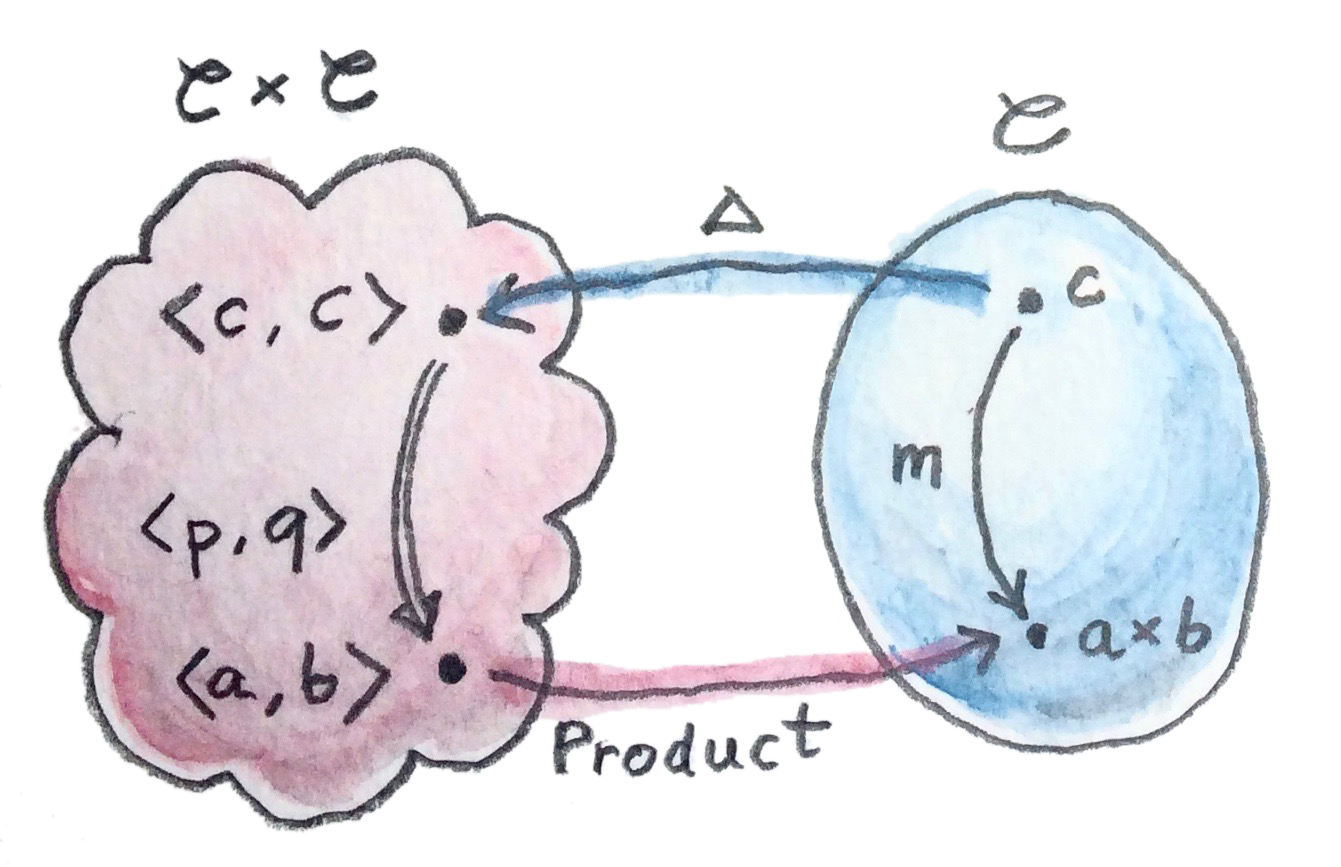
\includegraphics[width=3.12500in]{images/adj-product.jpg}
\end{figure}

\noindent
We still don't have a full adjunction. For that we first need our
\code{factorizer} to be invertible --- we are building an
\emph{isomorphism} between hom-sets. The inverse of the
\code{factorizer} should start from a morphism $m$ --- a
morphism from some object $c$ to the product object $a\times{}b$.
In other words, $m$ should be an element of:
\[\cat{C}(c, a\times{}b)\]
The inverse factorizer should map $m$ to a morphism
$\langle p, q \rangle$ in $\cat{C}\times{}\cat{C}$ that goes from
$\langle c, c \rangle$ to
$\langle a, b \rangle$; in other words, a morphism
that's an element of:
\[(\cat{C}\times{}\cat{C})(\Delta\ c, \langle a, b \rangle)\]
If that mapping exists, we conclude that there exists the right adjoint
to the diagonal functor. That functor defines a product.

In Haskell, we can always construct the inverse of the
\code{factorizer} by composing \code{m} with, respectively,
\code{fst} and \code{snd}.

\begin{Verbatim}
p = fst . m
q = snd . m
\end{Verbatim}
To complete the proof of the equivalence of the two ways of defining a
product we also need to show that the mapping between hom-sets is
natural in $a$, $b$, and $c$. I will leave this as
an exercise for the dedicated reader.

To summarize what we have done: A categorical product may be defined
globally as the \newterm{right adjoint} of the diagonal functor:
\[(\cat{C}\times{}\cat{C})(\Delta\ c, \langle a, b \rangle) \cong \cat{C}(c, a\times{}b)\]
Here, $a\times{}b$ is the result of the action of our right adjoint
functor $Product$ on the pair
$\langle a, b \rangle$. Notice that any functor from
$\cat{C}\times{}\cat{C}$ is a bifunctor, so $Product$ is a bifunctor. In
Haskell, the $Product$ bifunctor is written simply as
\code{(,)}. You can apply it to two types and get their product type,
for instance:

\begin{Verbatim}
(,) Int Bool ~ (Int, Bool)
\end{Verbatim}

\section{Exponential from Adjunction}

The exponential $b^a$, or the function object $a \Rightarrow b$, can be
defined using a \hyperref[function-types]{universal
construction}. This construction, if it exists for all pairs of objects,
can be seen as an adjunction. Again, the trick is to concentrate on the
statement:

\begin{quote}
For any other object $z$ with a morphism $g \Colon z\times{}a \to b$ \\
there is a unique morphism $h \Colon z \to (a \Rightarrow b)$
\end{quote}
This statement establishes a mapping between hom-sets.

In this case, we are dealing with objects in the same category, so the
two adjoint functors are endofunctors. The left (endo-)functor
$L$, when acting on object $z$, produces $z\times{}a$.
It's a functor that corresponds to taking a product with some fixed
$a$.

The right (endo-)functor $R$, when acting on $b$ produces
the function object $a \Rightarrow b$ (or $b^a$). Again, $a$ is
fixed. The adjunction between these two functors is often written as:
\[-\times{}a \dashv (-)^a\]
The mapping of hom-sets that underlies this adjunction is best seen by
redrawing the diagram that we used in the universal construction.

\begin{figure}[H]
\centering
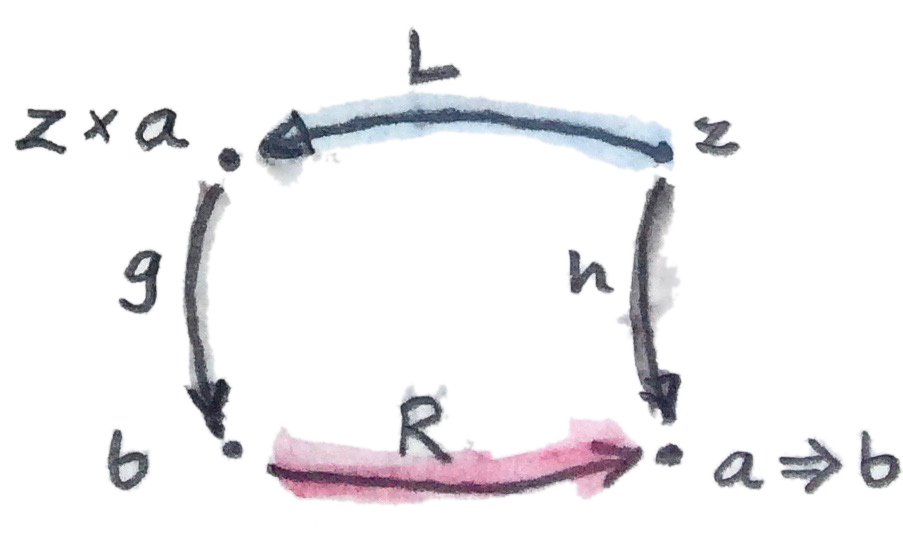
\includegraphics[width=60mm]{images/adj-expo.jpg}
\end{figure}

\noindent
Notice that the $eval$ morphism\footnote{See ch.9 on \hyperref[function-types]{universal
construction}.} is nothing else but the counit of
this adjunction:
\[(a \Rightarrow b)\times{}a \to b\]
where:
\[(a \Rightarrow b)\times{}a = (L \circ R) b\]
I have previously mentioned that a universal construction defines a
unique object, up to isomorphism. That's why we have ``the'' product and
``the'' exponential. This property translates to adjunctions as well: if
a functor has an adjoint, this adjoint is unique up to isomorphism.

\section{Challenges}

\begin{enumerate}
\tightlist
\item
  Derive the naturality square for $\psi$, the transformation
  between the two (contravariant) functors:
\begin{gather*}
a \to \cat{C}(L a, b) \\
a \to \cat{D}(a, R b)
\end{gather*}
\item
  Derive the counit $\varepsilon$ starting from the hom-sets isomorphism in
  the second definition of the adjunction.
\item
  Complete the proof of equivalence of the two definitions of the
  adjunction.
\item
  Show that the coproduct can be defined by an adjunction. Start with
  the definition of the factorizer for a coproduct.
\item
  Show that the coproduct is the left adjoint of the diagonal functor.
\item
  Define the adjunction between a product and a function object in
  Haskell.
\end{enumerate}